% !TEX program = xelatex
\documentclass[
  11pt,
  a4paper,
  oneside
]{article}

%%%%% Prepare Packages for Formatting
\usepackage{setspace}
\usepackage{geometry}
\geometry{tmargin=0.8in,bmargin=0.8in,lmargin=0.8in,rmargin=0.8in,headsep=0.0in,headheight=0.5in,foot=30.0pt}
\usepackage{float}
\usepackage{fancyhdr}         %draw header and foot
\usepackage[numbers,sort&compress]{natbib}

%%%%% CONFIG ABOUT HEADER AND FOOT
\pagestyle{fancy}
\fancyhf{}
\lhead{}
\chead{}
\rhead{{\footnotesize \textbf{Page \thepage}}}  %% PUT THE PAGE ON TOP RIGHT BUT NOT WORK
\lfoot{}
\cfoot{}
\rfoot{}  %% PUT THE PAGE ON TOP RIGHT BUT NOT WORK
% \setlength\parindent{0pt}

%%%%% Prepare Packages for Text
\usepackage[utf8]{inputenc}   %encoding
% \usepackage[T1]{fontenc}      %encoding
\usepackage{times}            %font
\usepackage[english]{babel}
\usepackage{titlesec}
\titleformat{\section}
{\normalfont\normalsize\bfseries}{\thesection.}{1em}{}
\usepackage{blindtext}
\usepackage[hyphens]{url}
% https://tex.stackexchange.com/a/238105
\usepackage[colorlinks=true,
            allcolors=blue]{hyperref}
\usepackage{graphicx}
\usepackage[no-math]{fontspec}
\usepackage{MnSymbol}
\usepackage{amsmath}
\usepackage{array}
\usepackage{ulem}
\usepackage{titling}
\usepackage{xltxtra}
\setmainfont{Arial}
\usepackage{svg}

%%%%% Helper Macros
%
\newcommand{\aLargeSquareToFill}{\fbox{\phantom{\rule{0.38in}{0.26in}}}}
%
\newcommand{\aLargeTickedSquare}{\fbox{\resizebox{0.38in}{0.26in}{$\checkmark$}} }
%
\newcommand{\titlepart}{\thispagestyle{empty}
\pdfbookmark[0]{Front Page}{Front Page}
\label{sec:frontpage}
\begin{center}
\textbf{Universidad Autonoma de Nuevo Leon\\
Facultad de Ingenieria Mecanica y Electrica\\
Posgrado de Ingenieria de Sistemas\\
\vspace{3ex}
RESEARCH PROJECT PROPOSAL}
\end{center}

\vspace{6ex}

Name of Candidate:\uline{
\phantom{xxxxxxxxxxxxxxxxxxx}
\theauthor
\hfill\phantom{x}}

\vspace{3ex}

Date of Admission to this programme:\uline{
\phantom{xxxxx}
\admissionDate
\hfill\phantom{x}}

\vspace{3ex}

\studyTimeMode

\leftskip=0.32in}


%%%%% Fill The Blanks with Personal Information
\author{Jose Alberto Benavides Vazquez}
\date{\today}
\title{Impact of the air pollutants in the population health in the Monterrey Metropolitan Area}
\newcommand{\admissionDate}{\today}
\newcommand{\studyTimeMode}{Full time mode}
% \newcommand{\studyTimeMode}{Part time mode}

%%%%% Begin Document
\hypersetup{
    pdfinfo={
    pdftitle=\thetitle,
    pdfauthor=\theauthor,
    pdfdate=\thedate
    }
}

\begin{document}

%%%%% Main Text
\titlepart

% \begin{abstract}
%     Brief summary of the proposal and its sections.
% \end{abstract}

\section{Project Title}
Impact of the air pollutants in the population health in the Monterrey Metropolitan Area.

\section{Introduction}
This study focuses on the impact that the air quality have in the population welfare primarily in the Monterrey Metropolitan Area between 2018 and 2019 obtained from the Comprehensive Environmental Monitoring System (abbreviated SIMA in Spanish from Sistema Integral de Monitoreo Ambiental) \citep{aireNL}. Also, it have been incorporated a database containing the hospital discharge records for Mexico over the same span of time from the open repository of the Department of Health of Mexico \cite{mexGobSS2020}.

As the atmosphere is result of the combination of $78\%$ of N$_2$,  $21\%$ of O$_2$ and $1\%$ of combined helium, water vapor, oxides, methane, noble gases, sulfides, ozone, ammonia, formaldehyde, and hydroxyl radical, can be defined that the air is \textit{polluted} when these concentrations are altered by human activities resulting in harmful environments to biological ecosystems \citep{thadEA2015}.

The human activities that cause pollution have been increasing over the years. Air quality became an urban problem since 1930 when a fog in Belgium was associated with the death of $63$ people and then in London during 1952 \citep{firket1936} when another fog caused $4,000$ deaths \citep{logan1953} being pneumonia the principal illness diagnosed in both cases. Its negative impact on health and general welfare concerned authorities that design regulations in order to minimize those undesirable effects. In 1981 it became an international problem when the CO concentrations were seen from space for the first time \citep{akimoto2003}. Such images show that the pollution was not only generated from expected sources, but from other unforeseen activities, and that the pollution generated in one place affected distant populations over time. 

Air pollution can be caused by events that impact the atmosphere, like forest fires, increased volcanic activity, animal and vegetable decomposition, climate change \citep{jacobEA2009}, etc. The main difference from natural and human pollutants is that the natural ones tend to occur far from large human populations and are less often than human sources of pollution, which are generally located in or near large human populations, and their emissions are more frequent. The main human sources of air pollution are associated with transportation, fuel combustion, and industrial processes \citep{fenger1999}.

The International Classification of Diseases (ICD)\footnote{The name of the diseases corresponding to the ICD code is obtained from \url{https://icd.who.int/browse10/2019/en}} is a code associated to diseases by their trends and statistical values, established by the \citeauthor{icd} \citep{icd}. It consists, generally, in a letter and three numbers between $0$ and $9$. For example, the code for \texttt{pneumonia due to staphylococcus} is \texttt{J152}. This system comprehends from the values \texttt{A00.0} to \texttt{Z99.9}, leaving the \texttt{U} letter for yet unknown sources. This classification was proposed by Farr at the end of the XIX century \cite{who2011}, and its purpose is to understand the causes of morbidity and mortality in order to improve the quality of life of the human population \cite{who2011}.

\section{Hypothesis}
The contamination levels reported can explain the statistically significant variations and trends of georeferenced data from health reports. Also, it is possible to automatize these relationships in an interactive and free web service.

\section{Project objectives}
\begin{itemize}
    \setlength\itemsep{-0.5em}
    \item Establish a clear and scientifically sustained relationship between air pollution and the human diseases that them can cause.
    \item Study the impact of the air pollution in the Metropolitan Monterrey Area during  2018 and 2019 in the health population.
    \item Choose or propose a methodology to calculate the causation between air pollution and associated human diseases.
    \item Identify the areas where they are more air pollution and establish a relationship between the people that live nearby those areas.
    \item Propose a rank to determine which air pollutants have the most direct effect in the human health.
    \item Propose pollution emission limits, scientifically justified, that can be used by organizations interested in this matter.
    \item Generate interactive and free tools that let people and specialist know the levels, relationships, risks, etc. related to the air pollutants studied.
\end{itemize}

\section{Research questions}
\begin{itemize}
    \setlength\itemsep{-0.5em}
    \item Is it possible to establish statistically significant relationships between air pollution and human diseases?
    \item What are the best methods to detect the causation between air pollution and human diseases?
    \item How to eliminate the climate and seasonal components from the relationship between air pollution and human diseases?
    \item Does the environmental and geographical factors can be used to predict the 
    amount of air pollution in an area and time?
    \item Which air pollutants cause more human diseases?
    \item Is it possible to establish short (days), medium (months) and large (years) interactions between air pollution and human diseases?
\end{itemize}

\section{Background and related literature}
The first correspondence to discuss relationship between air quality and human health was registered during December 1930 in Belgium, when a three-day fog s was declared to be the cause of death of 63 people --- during the fog, disease and death were observed to increase, whereas after its dissipation, the  figures normalized again \citep{firket1936}. Similarly, in December 1952, a four-day fog in London was associated with four thousand deaths \citep{logan1953}. The majority of the fog-related deaths were related to respiratory diseases.

In \citeyear{Lawther1959} \citeauthor{Lawther1959} \citep{Lawther1959} used a method to quantify the severity of respiratory illness based on their condition (negative numbers indicated they were recovered and positive numbers that they were getting worse). Then, he plotted a time series superposed with concentrations of two pollutants --- SO$_2$ and smoke --- and two weather variables --- temperature and humidity; he discovered that the pollutants bore a similarity to the severity whereas the climate ones did not.

During the 1970s, short-term exposure to different pollutants was studied \citep{HackneyEA1975, EhrlichEA1977, HackneyEA1978, LinnEA1978} with experiments that implied some ethical and legal considerations,  focusing on physiological analysis of the subjects. A compilation was published in by \citeauthor{Ferris1978} \citep{Ferris1978} who documented that the pollutants, in regulated concentrations, had a negative impact on health, primarily on respiratory diseases.

A set of methodologies are used to measure the relationships that are the focus of this study. They are \textbf{multiple regression analysis} \citep{Hyndman2018, Lebowitz1973, hasselblad1978, hatzakisEA1986} with variations in the distributions such as logistic regressions \citep{Korn1979}, \textbf{multivariate analysis} \citep{LaveEA1973, gottinger1983}, \textbf{auto regressive models} \citep{WeiEA1991}, \textbf{causality models} \citep{popescuEA2013} and \textbf{case-crossover approximations} \citep{Maclure1991, carracedoMartinezEA2009}.

\section{Methodology}
The study will focus in the \textbf{Monterrey Metropolitan Area (MMA)} between 2018 and 2019. The air quality samples in the are taken each hour from 13 sensors over the MMA that measure concentrations of \textbf{CO}, \textbf{NO}, \textbf{$\text{NO}_2$}, \textbf{$\text{O}_3$}, \textbf{$\text{SO}_2$}, \textbf{PM$_{10}$}, \textbf{PM$_{2.5}$}, and \textbf{atmospheric pressure}, \textbf{rainfall}, \textbf{relative humidity}, \textbf{solar radiation}, \textbf{temperature}, \textbf{wind velocity and direction}. This data is provided by the \textit{Sistema Integral de Monitoreo Ambiental de Nuevo León} (SIMA) \citep{aireNL}. The Mexican diseases data was obtained from the Mexican \textit{Department of Health} \citep{egresos} and contains information from all states and municipalities in Mexico such as \textbf{date of admission}, \textbf{egress date}, \textbf{age at the admission}, \textbf{gender}, \textbf{weight}, \textbf{height}, \textbf{ICD code upon arrived}, \textbf{ICD code upon diagnosis}, and \textbf{reason of egress}.

The air quality data needs to be interpolated because it contains imputed records. Different temporal interpolation techniques are used and compared \citep{Friedman1962}. Also, an spatio-temporal interpolation is performed to obtain the missing data values \citep{LiEA2002}. Both data sets are processed and converted to georeferenced time series \citep{Wei2019} that are stationary \citep{Hyndman2018} in order to establish their relationship by cross correlation \citep{derrickEA2004}, multiple regression analysis \citep{Brockwell2002}, vector autoregressive approaches, causality models \citep{popescuEA2013} and geographic interactions \citep{ComberEA2019}. The results are ranked by metrics like R$^2$, the Akaike (AIC), and the Bayesian (BIC) information criteria \citep{Albert2007}. Finally, it will be produced a web application that allow general and specialized population to interact with the data and obtain forecasts, interactions and visualizations of the models described.

\section{Expected results}
Univariate and multivariate analysis are performed on the time series from both the data sources of air quality and human diseases variables. Descriptive statistical results are expected to inform levels of pollutants and its levels according to local legislation (shown in Figure \ref{fig:ts_2018_pm10}) or timespans where more cases are reported (found in Figure \ref{fig:2017bymonth}). Causal analysis are based in causal diagrams (like the one on Figure \ref{fig:causation_example}). The causal tests have confidence intervals where $\alpha = 0.05$. For example, Figure \ref{fig:granger_test} shows the statistically significant results of a Granger test on $x$ causing $y$ variables in green. When there is a causal relationship between variables, mathematical models are able to find the relationships between the variables. Here, a vector autoregressive model is used to calculate the interactions between variables and its temporal lags. This results in equations where a variable can be explained from the most significant interactions and its coefficients. As an example, the \texttt{J} diseases depends on the interactions
\begin{equation*}
    Y_J = -1.96 a_{\texttt{J}:1} -3.81 a_{\texttt{J}:6} -0.89 a_{\text{PM10}:14} -6.71 a_{\texttt{J}:7} -1.31 a_{\text{PM10}:6} \ldots
\end{equation*}
where $a$ are the values of the variables and lags written as subindex in the form \texttt{variable:lag}.

\begin{figure}
    \centering
    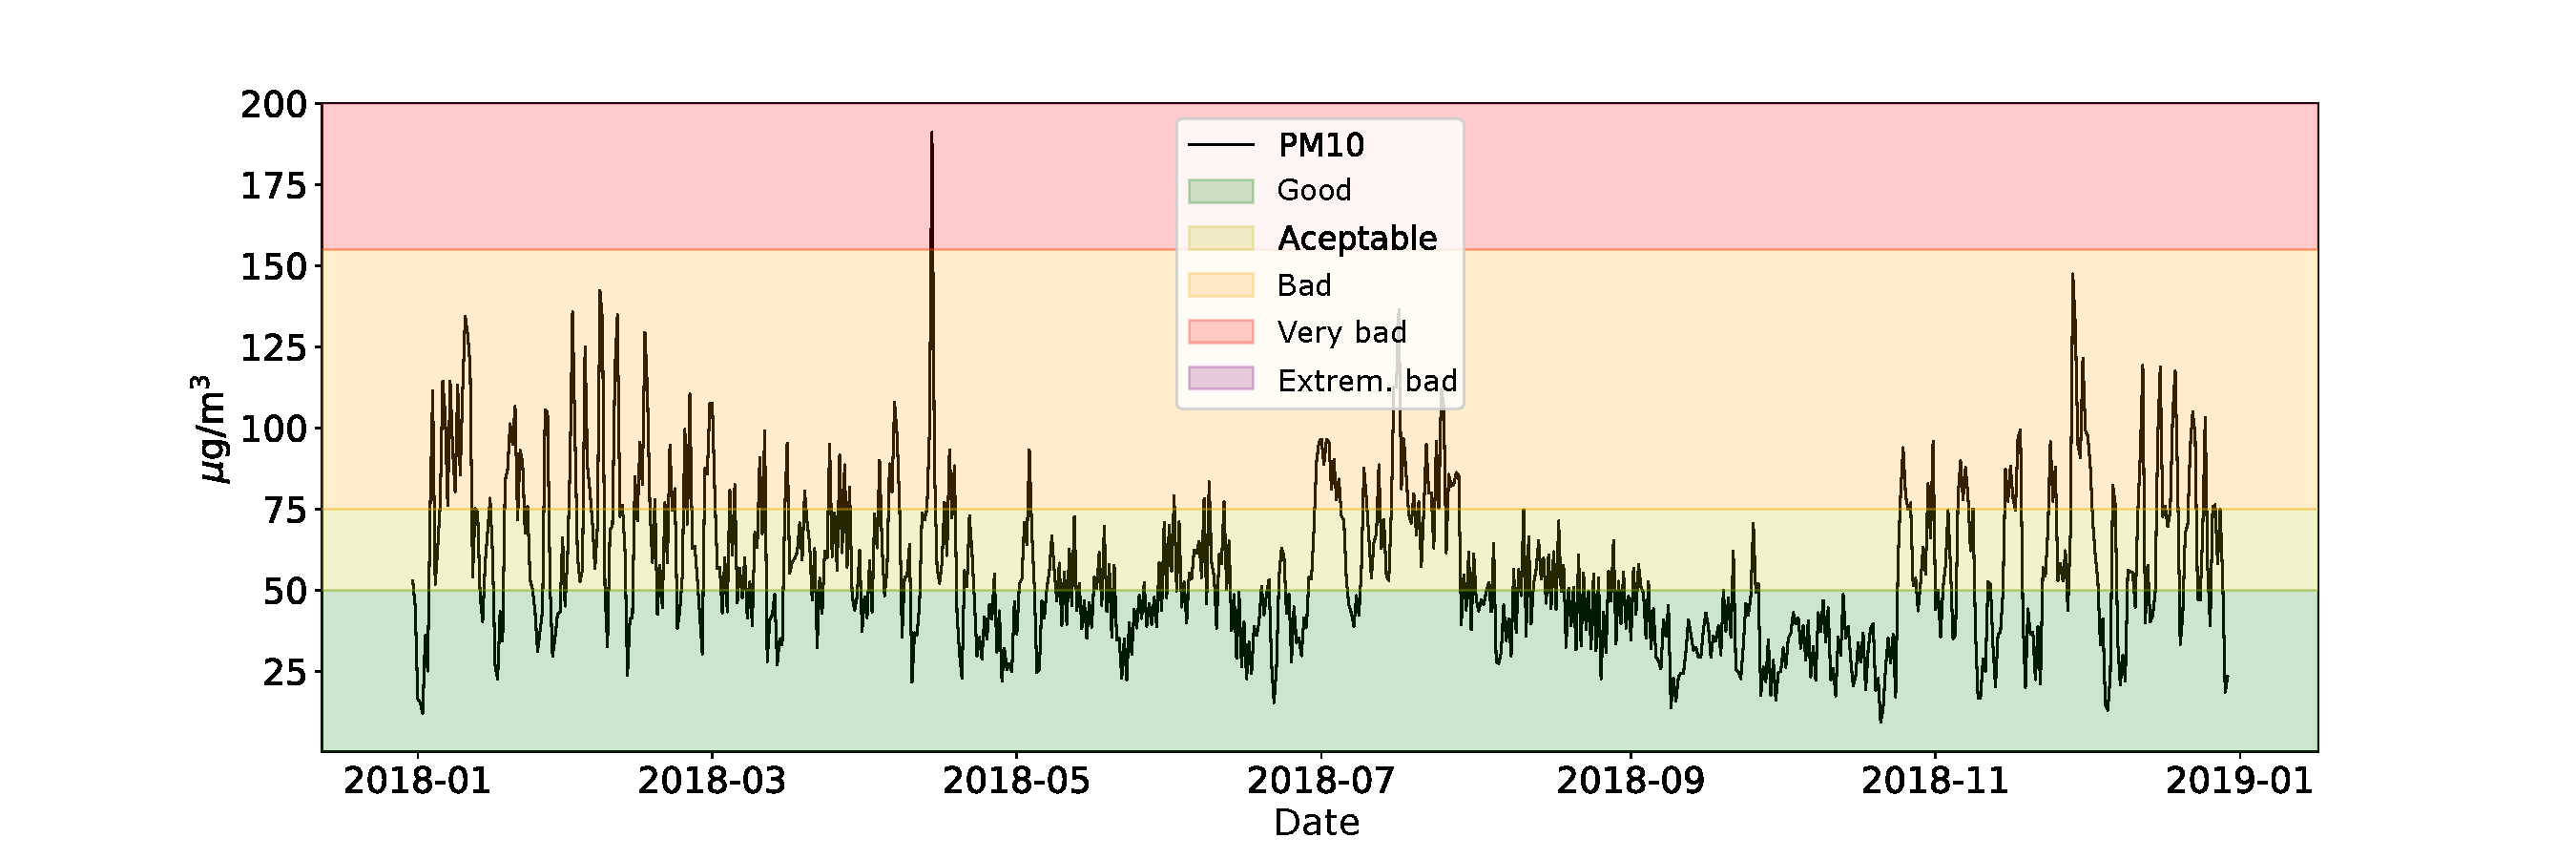
\includegraphics[width=1\textwidth]{figs/ts_2018_pm10.pdf}
    \caption{PM$_{10}$ 12-hour mean concentration for the MMA in 2018 displayed over the categorical ranges.}
    \label{fig:ts_2018_pm10}
\end{figure}

\begin{figure}
	\centering
        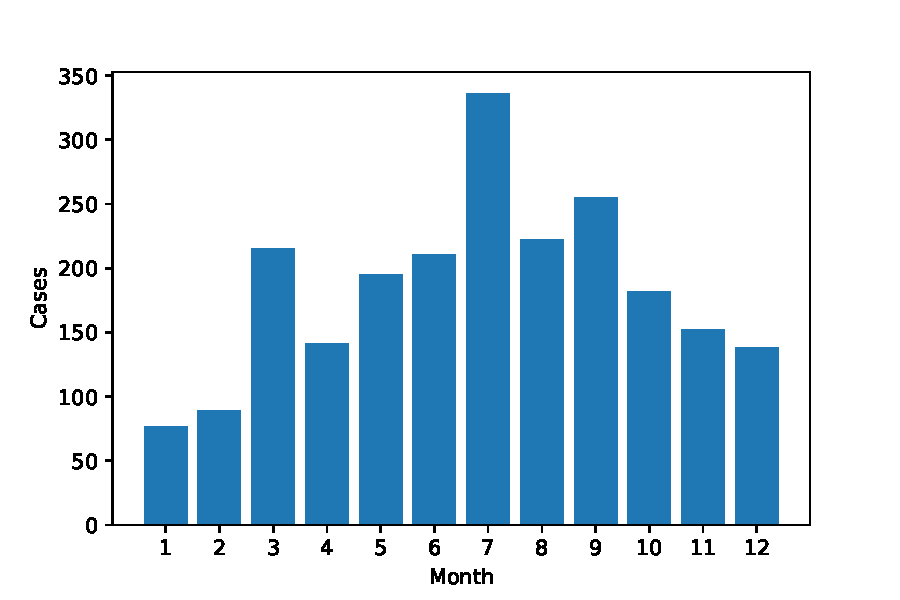
\includegraphics[width=0.9\textwidth]{figs/2017bymonth.pdf}
    \vspace*{-5mm}
	\caption{Bar diagram of the preprocessed records of patients from the MMA in 2017.}
	\label{fig:2017bymonth}
\end{figure}

\begin{figure}
    \centering
    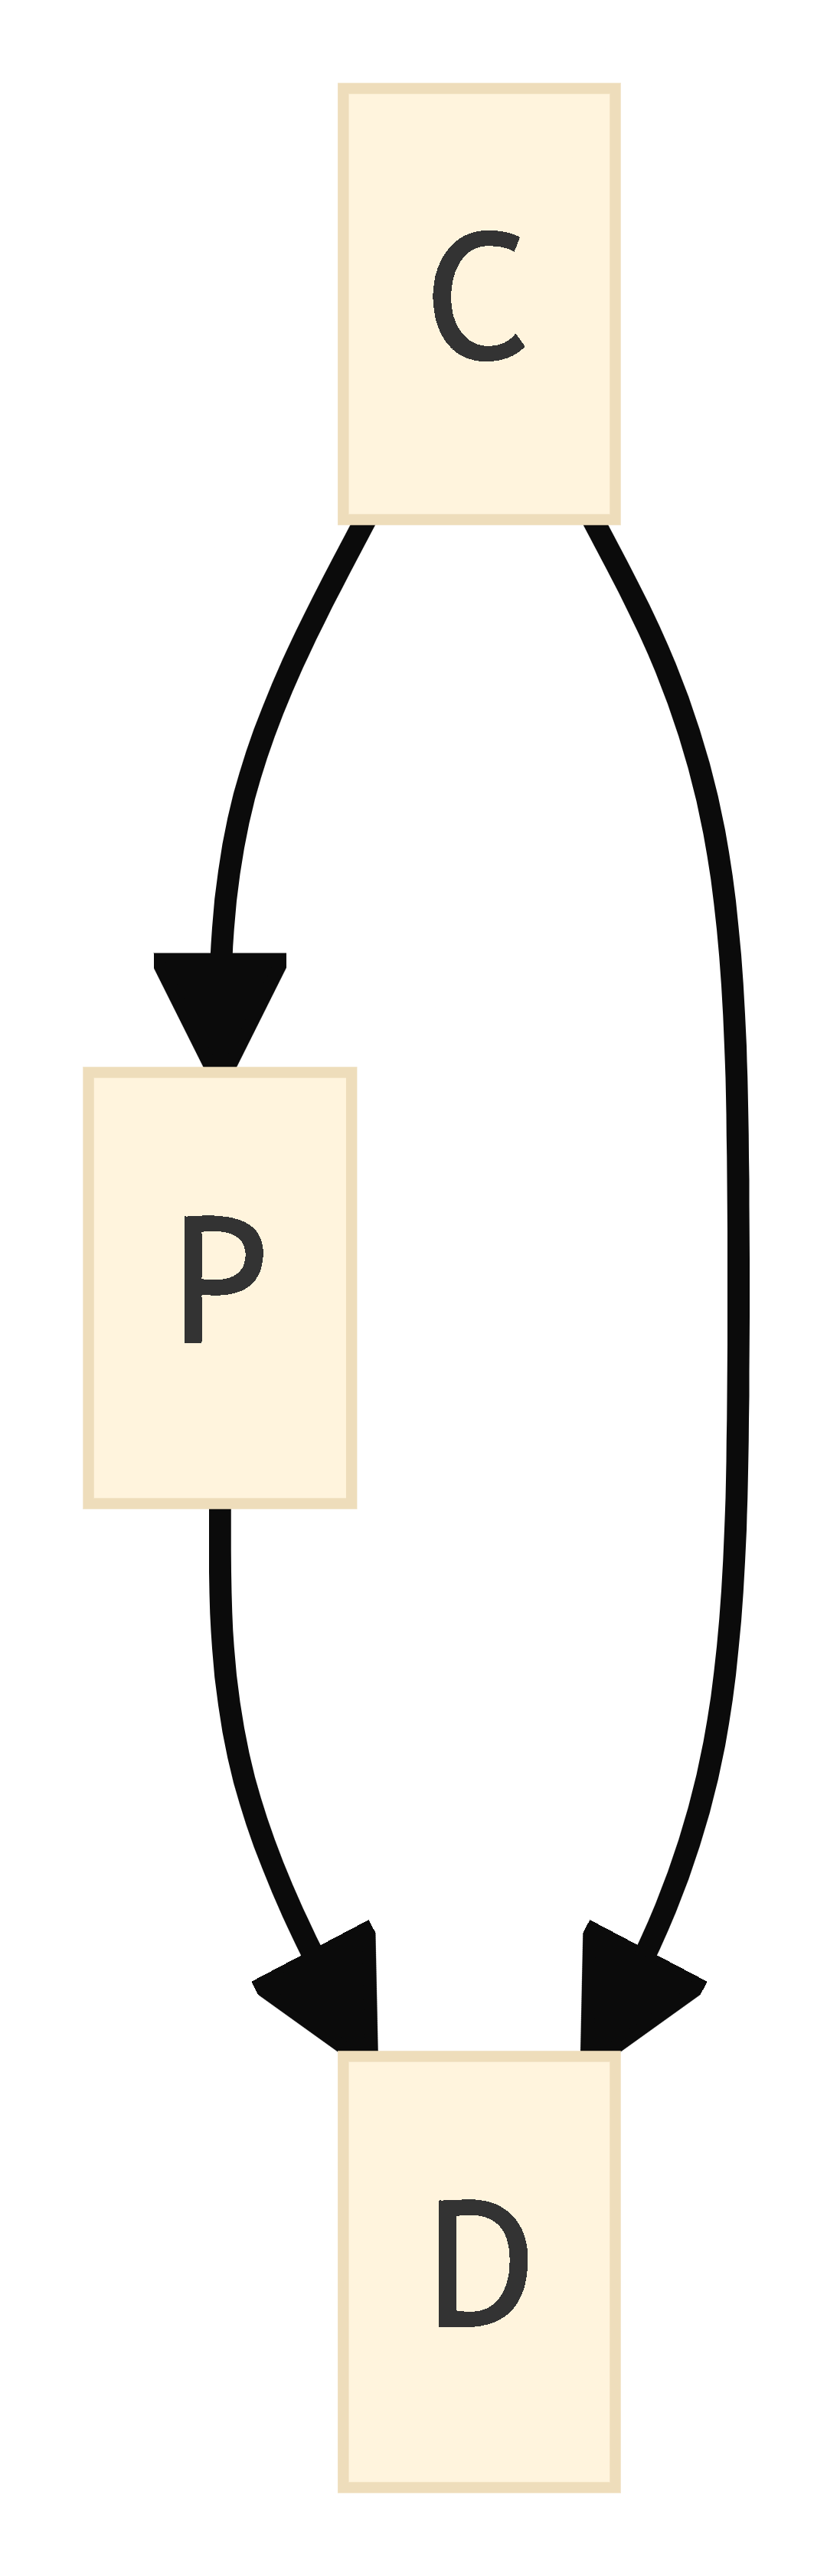
\includegraphics[width=0.1\textwidth]{figs/causation_example.png}
    \caption{Example of a causal diagram where pollutant P cause disease D, and both are caused by a confounding factor C.}
    \label{fig:causation_example}
\end{figure}

\begin{figure}
    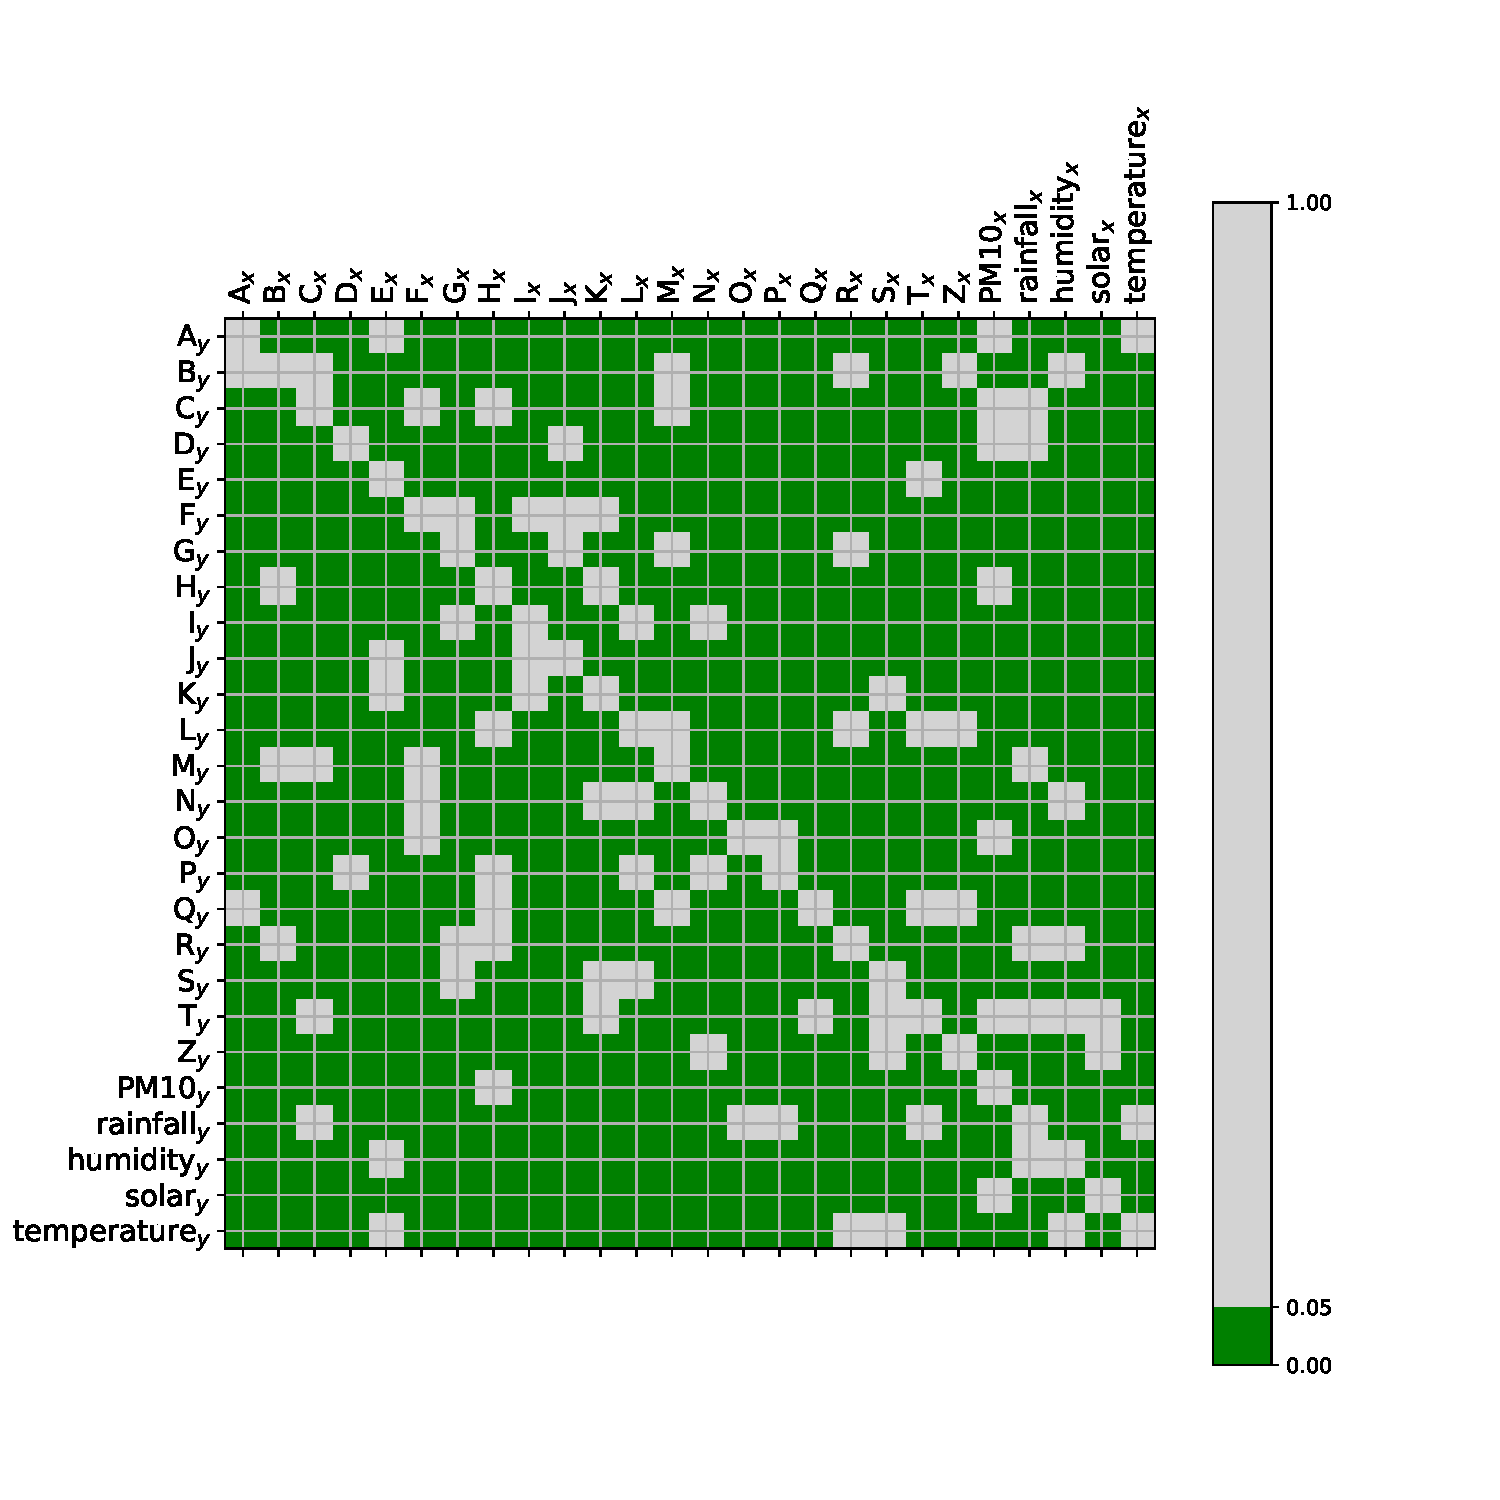
\includegraphics[trim={0 0 0 4em}, clip, width=1\textwidth]{figs/2018_granger.pdf}
    \caption{Granger causality test for $x$ (horizontal) variables causing $y$ variables (vertical).}
    \label{fig:granger_test}
\end{figure}

\section{Significance}
The relationship of air pollutants and human diseases have been widely studied. From those studies it is evident that the forecasting that can be produced it is relevant to the scientific community and other decision making agents. Nevertheless, the causation interactions of those factors are primarily studied in focus groups experiments where the ethical concerns limits the exploration. Mathematical causality models can bring a better understanding of the network of interactions between pollutants, diseases and confounding factors like weather conditions such as temperature, atmospheric pressure and so on, supporting the possibility of simulations that extends the ethical concerns limits discussed.

\section{Project schedule}
% https://tex.stackexchange.com/a/40521
\begin{sloppypar}
The Gantt diagram of this project can be accessed in  \url{https://aulaplus.notion.site/c5e2f4f3b8004123ac356811e598a63e?v=34166671ce074e6499778146b40b3462}.
\end{sloppypar}
\bibliographystyle{plainnat}
\bibliography{../biblio}

\end{document}